\documentclass{kti}

% ----------------------------------------
% Metadata
% ----------------------------------------
\faculty{KAMPUS UPI DI CIBIRU}
\program{Program Studi REKAYASA PERANGKAT LUNAK}
\title{Implementasi Arsitektur Sistem Berbasis High Availability untuk Mencapai Auto Scalability dan Zero Downtime Deployment pada Platform GCP (Studi Kasus: EMODU)}
\author{Muhamad Fadil}
\email{fadilmuh22@student.upi.edu}
\studentid{2109994}
\yearsubmit{2024}

% In Thesis:
% \titleen{}
% \monthsubmit{January}
% \firstsupervisorname{}
% \firstsupervisorid{}
% \secondsupervisorname{}
% \secondsupervisorid{}
% \departmentheadname{}
% \departmentheadid{}

% TODO: cek kembali secara menyeluruh
\hyphenation{meng-gu-na-kan seg-men-ta-tion me-ngu-kur me-nye-sat-kan me-nge-na-li pe-nge-na-lan pe-ne-ra-pan ek-strak-si di-man-fa-at-kan eks-pre-si re-le-van ha-ra-pan men-cer-min-kan meng-hu-bung-kan key-board di-u-sul-kan di-la-ku-kan di-gu-na-kan me-nge-na-kan di-sip-lin neu-ron pe-la-ti-han di-ru-mus-kan craw-ling en-hance-ment akan ber-da-sar-kan me-nga-dop-si di-sim-pan me-ne-rap-kan me-ning-kat-kan ke-se-lu-ru-han me-lan-jut-kan di-ten-tu-kan di-per-li-hat-kan ke-sa-la-han dis-gust weighted di-per-lu-kan neu-tral men-ja-jar-kan ka-nan net-work en-sem-ble}

\addbibresource{references.bib}
\emergencystretch=1em

\begin{document}

\frontmatter
% ----------------------------------------
% Halaman judul
% ----------------------------------------
\cover

% In Thesis:
% % ----------------------------------------
% Halaman hak cipta
% ----------------------------------------
% \copyright

% ----------------------------------------
% Halaman pengesahan
% ----------------------------------------
% \approval

% ----------------------------------------
% Halaman pernyataan keaslian dan bebas
% plagiarisme
% ----------------------------------------
% \statementcontent{Saya menyatakan bahwa skripsi berjudul ``Pengenalan Emosi Manusia Menggunakan \textit{Log-Gabor Convolutional Networks} Melalui Pendekatan \textit{Facial Region Segmentation}'' ini adalah benar karya saya sendiri. Dan saya tidak melakukan tindakan plagiat yang menyalahi etika dalam karya tulis ilmiah. Apabila saya terbukti bersalah, maka saya bersedia untuk memperbaiki diri, meminta maaf kepada pihak yang bersangkutan dan menanggung setiap sanksi yang berlaku.}
% \statement

% ----------------------------------------
% Halaman ucapan terima kasih/persembahan
% ----------------------------------------
% \acknowledgmentcontent{Untuk ibu, bapak\\dan adik-adikku tercinta.}
% \acknowledgment

% ----------------------------------------
% Kata pengantar
% ----------------------------------------
% \prefacecontent{Segala puji bagi Allah \textit{Subh\=anahu wa Ta’\=ala}, yang dengan nikmat-Nya maka sempurnalah segala kebaikan. Tiada daya dan upaya kecuali hanya dari-Nya. Hanya dengan memohon pertolongan-Nya, penulis dapat menyelesaikan skripsi berjudul ``Pengenalan Emosi Manusia dengan \textit{Log-Gabor Convolutional Networks} Melalui Pendekatan \textit{Facial Region Segmentation}'' ini tepat waktu. Skripsi ini disusun dalam rangka memenuhi sebagian syarat memperoleh gelar Sarjana S-1 Jurusan Ilmu Komputer di Universitas Pendidikan Indonesia.

% Pada kenyataannya, skripsi ini bukan merupakan kredit tersendiri bagi penulis. Melainkan merupakan upaya murni kolaboratif dengan berbagai pihak selama penulis belajar di bangku perkuliahan. Setelah memulai dengan mengucapkan syukur kepada Allah \textit{Subh\=anahu wa Ta’\=ala} di atas segalanya, penulis ingin mengucapkan terima kasih yang tulus kepada kedua pembimbing skripsi ini, bapak Yaya Wihardi dan bapak Wawan Setiawan, karena telah bersedia dengan sepenuh hati membimbing penulis dalam menyelesaikan skripsi ini.

% Sejak diberikan kesempatan oleh bapak Yaya untuk bergabung bersama beliau, bapak Wawan, ibu Enjun Junaeti dan keempat anggota lain dalam riset \textit{smart classroom}, penulis merasa lebih beruntung dari kebanyakan teman-teman lain. Selama melakukan riset bersama-sama, penulis telah banyak belajar dari berbagai tahap yang telah dilalui.

% Penulis ingin mengucapkan terima kasih sebanyak-banyaknya kepada bapak Yaya sebagai mentor terbaik. Selama melakukan bimbingan, beliau telah memberikan sebuah advis kepada penulis bahwa skripsi yang bagus adalah yang selesai. Ketika skripsi itu harus tertunda penyelesaiannya karena ingin serba perfek, maka akan banyak peluang yang mungkin terlewatkan. Terus terang, penulis sangat menyukai bagaimana beliau mengumpulkan setiap mahasiswanya di ruangan yang sama untuk melakukan bimbingan pekanan. Dengan begitu, penulis telah mendapatkan berbagai masukan dan pandangan yang berbeda dari beliau sendiri dan teman-teman saat itu. Selama mengikuti kelas, penulis telah banyak belajar dari beliau khususnya mengenai \textit{computer vision} dan \textit{image processing}. Bagi penulis, beliau termasuk salah satu dosen yang paling cakap dalam mengajar. Sebagai salah satu anggota laboratorium Kecerdasan Buatan dan Robotika, beliau telah meneladani penulis untuk memiliki loyalitas dan kedisplinan yang tinggi.

% Juga terima kasih kepada bapak Wawan yang telah mempercayai penulis sebagai salah satu anggota riset \textit{smart classroom} yang beliau ketuai. Tanpa dukungan yang besar dari beliau, penulis tidak akan memiliki kesempatan untuk dapat bermalam di kampus dan menuntaskan proyek akhir robotika.

% Penulis merasa sangat bersyukur telah diberikan kesempatan dan kepercayaan dalam mengajar sebagai asisten dari ibu Rani Megasari di kelas Basis Data, bapak Yudi Wibisono di kelas Sistem Basis Data, bapak Herbert Siregar di kelas Pemrograman Visual dan bapak Eddy Prasetyo Nugroho di kelas Rekayasa Perangkat Lunak. Terima kasih juga kepada teman-teman yang telah menjadi partner mengajar yang kompeten. Dengan mengajar, penulis tidak hanya mendapatkan pengetahuan yang lebih luas dan mendalam mengenai bahan ajar yang disampaikan, namun juga mendapatkan keluasan untuk meningkatkan kemampuan mengajar dan berbicara di depan kelas. Penulis menjadi mengerti bahwa menempatkan diri bukan sebagai pengajar, akan tetapi sebagai partner bagi para studen, penting dilakukan dalam mengajar di kelas. Hubungan emosional yang baik sedikit banyak mempengaruhi motivasi mereka dalam mengikuti kelas.

% Penulis merasa sangat beruntung telah memiliki dosen-dosen yang istimewa. Sangat menyenangkan mendengarkan mereka saling menceritakan kisah inspiratif satu sama lain. Selain yang sudah disebutkan di atas, penulis ingin berterima kasih lebih khusus kepada ibu Rosa Ariani Sukamto yang telah mengajarkan penulis untuk tidak perlu menjadi orang lain, untuk selalu jujur dalam berlaku dan untuk selalu berjuang juga tidak malu dalam belajar. Juga kepada bapak Yudi yang telah mengajarkan penulis untuk tidak takut berbuat kesalahan dalam belajar dan untuk tidak berhenti belajar sebelum mampu menghasilkan buah karya. Juga kepada bapak Herbert Siregar yang telah mengajarkan penulis untuk selalu belajar memahami sesuatu secara mendasar dan untuk selalu memiliki etos juga etika dalam bekerja. Juga kepada bapak Eddy yang telah mengajarkan penulis untuk selalu menilai sesuatu secara adil juga lugas. Juga kepada ibu Enjun yang telah mengajarkan penulis untuk selalu mengutamakan disiplin dalam berlaku dan untuk selalu menghargai usaha orang lain. Juga kepada dosen-dosen lain yang tidak dapat disebutkan satu per satu. Namun, satu hal yang dapat dipastikan bahwa penulis telah belajar banyak sekali makna dari mereka semua. Jika diperbolehkan, penulis ingin selalu dapat duduk setidaknya satu kali lagi di hadapan mereka untuk mendengarkan dan mencatat beberapa pelajaran terakhir.

% Tidak lupa, penulis juga ingin mengucapkan terima kasih kepada teman-teman yang telah memberikan warna dan menyulap setiap kebersamaan kami dalam belajar di kelas menjadi sangat menyenangkan dan tidak akan pernah tergantikan. Yang telah membuat kenangan dalam ruang-ruang kelas tidak akan pernah sama jika tanpa mereka. Secara istimewa, penulis ingin berterima kasih sebanyak-banyaknya kepada Muhammad Faris Muzakki dan Yahya Firdaus yang telah menjadi partner dalam banyak pekerjaan. Juga kepada Ammar Ashshiddiqi, Reyhan Fikri Dzikriansyah, Teguh Arianto,, Adnan Khairi As., Asep Saepul Ahmad, I. G. N. Agung A. A. W., dan Genta Satria A. P. sebagai teman-teman terdekat penulis dalam menjalani kehidupan di kampus. Juga kepada kakak-kakak tingkat yang telah bersedia menjawab dan memandu penulis dengan begitu tulus dan tanpa pamrih dalam belajar.

% Setiap momen yang penulis habiskan bersama teman-teman seperjuangan adalah menyenangkan dan tidak akan tergantikan. Di sisi lain, setiap momen duduk mencatat dan mengacungkan tangan bertanya mengenai setiap pelajaran yang disampaikan oleh dosen-dosen yang berdedikasi juga tidak akan terlupakan. Bersama dengan mereka semua, kami telah saling berbagi banyak pengetahuan dan cerita.

% Tanpa henti-hentinya, penulis juga bersyukur telah diberikan keluarga yang selalu menjadi orang-orang yang paling pertama dan paling setia dalam mendukung setiap keputusan penulis. Mereka adalah abi Ahmad Djunaedi Sastradinata, umi Desy Rosika Natalia, Ahmad Faaiz Al-Auza'i, Salma Kaisan Syauqi dan Kaisa Rifqa Ghassani. Tanpa doa dan dukungan dari mereka semua, penulis tidak akan mampu berdiri dan melangkah di atas kaki sendiri menuju perjalanan yang penuh dengan kebahagiaan.

% Terakhir, penulis ingin berterima kasih kepada bapak Lala Septem Riza selaku Ketua Departemen Pendidikan Ilmu Komputer Universitas Pendidikan Indonesia, ibu Rani selaku Ketua Program Studi Ilmu Komputer Universitas Pendidikan Indonesia serta semua dosen penguji proposal juga laporan akhir skripsi ini.

% Demikian pengantar ini dibuat dengan sungguh-sungguh. Penulis berharap bahwa pekerjaan ini dapat bermanfaat bagi penulis sendiri dan seluruh pembaca budiman. \textit{At last but not least}, penulis menyatakan secara terbuka untuk menerima segala masukan dalam menyempurnakan skripsi ini.}
% \preface

% ----------------------------------------
% Abstrak
% ----------------------------------------
% \abstractcontent{Pengenalan emosi manusia secara otomatis dapat bermanfaat pada sektor-sektor terkait komputasi afektif. Penelitian ini merupakan penelitian pertama yang mengadopsi teknik \textit{facial region segmentation} (FRS) pada arsitektur \textit{Log-Gabor Convolutional Networks} (Log-GCNs) dalam membangun model menggunakan set data gambar wajah nonfrontal, FER-2013. Dengan menggunakan deteksi \textit{facial landmark}, daerah fitur wajah tertentu dapat disegmentasi menjadi dua-tiga bagian. Setiap bagian dapat dilatih baik secara individu maupun bersamaan menggunakan teknik \textit{network ensemble}, di mana sejumlah arsitektur GCN yang identik tergabung di dalamnya. Hasil eksperimen membuktikan bahwa Log-GCN dengan FRS berhasil mengungguli \emph{baseline} dengan augmentasi data melalui peningkatan akurasi sebesar 6,07\%.}
% \abstractkeywords{Rekognisi emosi; rekognisi ekspresi wajah; FER; segmentasi daerah wajah; \textit{deep convolutional neural network}; jaringan ansambel.}

% \abstractencontent{Automatic recognition of human emotions can be useful in sectors related to affective computing. We believe that it is the first study to adopt facial region segmentation (FRS) techniques on the Log-Gabor Convolutional Networks (Log-GCNs) architecture in order to build a model that using the non-frontal face dataset images, FER-2013. By using facial landmarks detection, certain facial feature areas can be segmented into two-three parts. Each region can be trained either individually or together using network ensemble techniques, where a number of identical GCN architectures are combined. The experimental results prove that Log-GCN with FRS successfully outperformed the baseline with data augmentation through an increase in accuracy of 6.07\%.}
% \abstractenkeywords{Emotion recognition; facial expression recognition; FER; facial region segmentation; deep convolutional neural network; network ensemble.}
% \abstract


% ----------------------------------------
% Daftar isi
% ----------------------------------------
\addcontentsline{toc}{chapter}{DAFTAR ISI}
\tableofcontents

% ----------------------------------------
% Daftar tabel
% ----------------------------------------
\listoftables
\addcontentsline{toc}{chapter}{DAFTAR TABEL}

% ----------------------------------------
% Daftar gambar
% ----------------------------------------
\listoffigures
\addcontentsline{toc}{chapter}{DAFTAR GAMBAR}

% ----------------------------------------
% Daftar lampiran
% ----------------------------------------
% [TODO]

\newpage
\mainmatter
% ----------------------------------------
% Isi
% ----------------------------------------
\chapter{Pendahuluan}
\section{Latar Belakang}
\qquad Kemajuan teknologi informasi saat ini memungkinkan pengembangan berbagai inovasi dalam bidang pendidikan, termasuk implementasi teknologi berbasis AI untuk meningkatkan interaktivitas dan efektivitas pengajaran. Salah satu aspek penting dalam proses pembelajaran adalah kemampuan seorang pendidik untuk memahami keadaan emosional siswa, yang kerap tercermin melalui ekspresi wajah. Kemampuan ini, jika dapat diukur secara otomatis dan real-time, dapat membantu pendidik dalam menyesuaikan metode pengajaran dan menciptakan suasana belajar yang lebih kondusif.

Aplikasi berbasis Face Recognition dan analisis ekspresi wajah menjadi relevan untuk mengatasi tantangan ini. Teknologi ini memungkinkan sistem untuk mengidentifikasi ekspresi wajah siswa, seperti senang, sedih, atau bingung, yanlg kemudian dapat disampaikan kepada pendidik sebagai indikator untuk menilai suasana kelas secara keseluruhan. Penggunaan komunikasi socket dalam sistem ini, yang memungkinkan transfer data secara langsung dan berkesinambungan antara klien dan server, memfasilitasi proses analisis ekspresi wajah secara real-time dan memastikan data tersampaikan dengan cepat dan akurat \cite{ogundeyiWebSocketRealTime2019}.

Namun, ada beberapa tantangan teknis dalam mengoptimalkan sistem seperti ini, khususnya dalam hal performa sistem dan kecepatan pemrosesan. Penggunaan socket communication harus dioptimalkan agar dapat menangani lalu lintas data yang besar dengan latensi rendah. Di sisi lain, algoritma analisis ekspresi wajah harus dapat berjalan secara efisien tanpa membebani perangkat pengguna (Phankokkruad et al., 2016). Penelitian ini bertujuan untuk mengoptimalkan sistem analisis ekspresi wajah pada aplikasi pengajaran berbasis Face Recognition dan socket communication, sehingga dapat memberikan hasil analisis secara real-time dan meminimalkan gangguan teknis yang dapat mengurangi efektivitas pengajaran.

\section{Rumusan Masalah}

{Berdasarkan latar belakang yang telah dijelaskan, rumusan masalah dalam
penelitian ini adalah sebagai berikut:}

\begin{enumerate}
% \tightlist
\item
  {Bagaimana mengoptimalkan sistem analisis ekspresi wajah secara
  Real-Time pada aplikasi pengajaran berbasis Face Recognition?}
\item
  {Bagaimana pemanfaatan Socket Communication dapat meningkatkan
  kecepatan dan keakuratan dalam pengiriman data ekspresi wajah secara
  Real-Time?}
\item
  {Bagaimana mengukur efektivitas optimasi yang diterapkan terhadap
  kinerja aplikasi?}
\end{enumerate}

\section{Tujuan}

{Penelitian ini bertujuan untuk:}

\begin{enumerate}
% \tightlist
\item
  {Mengoptimalkan sistem analisis ekspresi wajah pada aplikasi
  pengajaran berbasis real-time menggunakan Face Recognition dan Socket
  Communication.}
\item
  {Meningkatkan kecepatan dan keakuratan pengiriman data ekspresi wajah
  dalam aplikasi pengajaran melalui implementasi Socket Communication.}
\item
  {Mengidentifikasi tantangan dan mengembangkan solusi dalam optimasi
  sistem real-time untuk pengajaran interaktif.}
\item
  {Mengevaluasi efektivitas dari optimasi yang diterapkan terhadap
  performa dan kualitas aplikasi dalam mendukung proses pengajaran.}
\end{enumerate}

\section{Manfaat}

{Adapun manfaat yang diharapkan dari penelitian ini adalah sebagai
berikut:}

\begin{enumerate}
% \tightlist
\item
  {Menyediakan kontribusi keilmuan di bidang pengenalan wajah dan
  komunikasi data real-time dalam konteks pendidikan, serta sebagai
  referensi bagi penelitian selanjutnya.}
\item
  {Aplikasi hasil penelitian ini diharapkan dapat membantu pendidik
  dalam memahami ekspresi dan kondisi emosional siswa secara lebih
  efektif, sehingga dapat meningkatkan interaktivitas dan kualitas
  pembelajaran.}
\item
  {Menjadi referensi bagi pengembangan sistem serupa yang memerlukan
  optimasi pengiriman data real-time dan analisis ekspresi wajah dala}{m
  konteks yang lebih luas.}
\end{enumerate}

\section{Batasan}

{Untuk memastikan fokus penelitian dan hasil yang terarah, penelitian
ini memiliki beberapa batasan sebagai berikut:}

\begin{enumerate}
% \tightlist
\item
  {Aplikasi ~akan dibatasi pada penggunaan teknologi face recognition.
  Menggunakan komunikasi data melalui REST API dan Socket Communication
  pada aplikasi berbasis web.}
\item
  {Pengujian dilakukan dalam lingkungan simulasi kelas kecil, dengan
  jumlah pengguna yang terbatas.}
\item
  {Sistem hanya akan diimplementasikan pada platform WEB Desktop dengan
  kamera, dan tidak diuji pada perangkat mobile.}
\end{enumerate}

\chapter{Kajian Pustaka}

\section{State of The Art}

\vspace{-1cm}
\begin{longtable}[t]
{@{}
  |>{\raggedright\arraybackslash}p{(\columnwidth - 6\tabcolsep) * \real{.25}}
  |>{\raggedright\arraybackslash}p{(\columnwidth - 6\tabcolsep) * \real{.25}}
  |>{\raggedright\arraybackslash}p{(\columnwidth - 6\tabcolsep) * \real{.25}}
  |>{\raggedright\arraybackslash}p{(\columnwidth - 6\tabcolsep) * \real{.25}}|
@{}}
\endhead
\endlastfoot

\caption{State of The Art} \\

\hline
\textbf{Judul Penelitian} &
\textbf{Metrik} &
\textbf{Metode Penelitian} &
\textbf{Hasil} 

\\ \hline
{A Real-time Face Recognition for Class Participation Enrollment System Over WebRTC} &
{Akurasi deteksi wajah, ~Attendance reliability, performa Real-Time.} &
{Implementasi pengenalan wajah berbasis WebRTC untuk sistem kehadiran kelas, dengan evaluasi akurasi dan kecepatan respons.} &
{Sistem terbukti efektif untuk mencatat kehadiran kehadiran siswa dan dapat memotivasi siswa untuk hadir di kelas.} 

\\ \hline
{Real Time Face Detection and Facial Expression Recognition: Development and Applications to Human Computer Interaction.} &
{Akurasi deteksi wajah, performa Real-Time.} &
{Deteksi wajah dengan cascade fitur dan pengenalan ekspresi menggunakan Gabor-SVM, diuji pada dataset Cohn-Kanade.} &
{Mencapai akurasi 93\% dalam deteksi ekspresi real-time dan telah diimplementasikan di berbagai platform untuk interaksi manusia-mesin.}

\\ \hline
{Real time Face Detection and Optimal Face Mapping for Online Classes} &
{Akurasi deteksi wajah, ~Attendance reliability, Real-Time Performance.} &
{Perbandingan algoritma Local Binary Pattern Histogram (LBPH) dan Convolutional Neural Network (CNN) untuk pengenalan wajah serta Haar Cascade untuk deteksi wajah.} &
{Algoritma CNN memiliki akurasi 95\%, lebih tinggi dibandingkan LBPH (78\%), menunjukkan keunggulan untuk kehadiran real-time dalam kelas online.}

\\ \hline
{Web Application Development for Biometric Identification System Based on Neural Network Face Recognition} &
{Akurasi deteksi wajah, System Response.} &
{Pengembangan aplikasi web berbasis neural network untuk identifikasi wajah dengan arsitektur MVC dan pengujian performa modul.} &
{Kompleks identifikasi biometrik berhasil diterapkan di lingkungan keamanan seperti bandara dengan akurasi tinggi.} 

\\ \hline
{Web Front-End Realtime Face Recognition Based on TFJS} &
{Latency, Kecepatan deteksi wajah.} &
{Implementasi pengenalan wajah di browser menggunakan TensorFlow.js dan pengujian pada berbagai skenario untuk mengurangi beban server.} &
{Sistem pengenalan wajah Real-Time di sisi Client berhasil menurunkan latensi dan beban Server, menunjukkan respons yang dapat diterima pengguna.} 

\\ \hline
{Web Performance Optimization Techniques for Biodiversity Resource Portal} &
{Efficiency Score, Load Lime, Page Rank, End-to-End Performance Indicators.} &
{Analisis sebelum dan pasca-optimasi menggunakan teknik Web Performance Optimization (WPO), dinilai dengan GTmetrix.} &
{Peningkatan signifikan dalam performa portal, dari Grade F (13\%) menjadi Grade B (82\%) setelah optimasi.}

\\ \hline
{WebSocket in real time application} &
{Latency, Efficiency, Data Transmission Reliability } &
{Analisis performa WebSocket dibandingkan dengan HTTP
long polling dan server-sent events untuk aplikasi real-time.} &
{WebSocket memberikan performa yang lebih baik dalam latensi dan efisiensi jaringan, mendukung pertukaran data dua arah yang lebih halus untuk aplikasi real-time.} 

\\ \hline
{PROPOSED} &
{Memory Usage, System Responses, Real-Time Performance.} &
{Uji coba aplikasi dan web server pada aplikasi web virtual meeting untuk menguji performa.} &
{Menganalisis cara meengoptimalkan kecepatan, keakuratan, dan efektivitas sistem analisis ekspresi wajah berbasis face recognition dan socket communication} 

\\ \hline

\end{longtable}

\newpage

\section{Deteksi Ekspresi}
Deteksi ekspresi wajah adalah proses analisis dan interpretasi ekspresi wajah manusia melalui perangkat lunak untuk mengenali emosi, seperti senang, sedih, bingung, dan fokus. Teknologi ini sering didasarkan pada face recognition yang mengidentifikasi fitur-fitur wajah melalui berbagai teknik seperti pengenalan pola, analisis tekstur, dan deep learning \parencite{archanaRealTimeFace2022}. Dalam aplikasi pengajaran berbasis real-time, deteksi ekspresi wajah memungkinkan pengajar untuk memahami respons siswa dengan cepat, mendukung interaksi yang lebih responsif dan efektif dalam pembelajaran \parencite{archanaRealTimeFace2022}.

\section{Socket Communication}
Socket communication adalah metode yang digunakan untuk memungkinkan transfer data secara real-time antara client dan server. Teknologi ini memanfaatkan protokol TCP/IP atau WebSocket untuk mempertahankan koneksi yang persisten, memungkinkan aplikasi untuk mengirim dan menerima data secara cepat dan efisien. Dalam konteks aplikasi pengajaran berbasis real-time, socket communication berperan penting untuk memastikan bahwa data terkait ekspresi wajah siswa dapat dikirimkan secara Real-Time ke server dan disampaikan kepada pengajar yang memungkinkan minimnya Latency dan Network Traffic di sistem \parencite{ogundeyiWebSocketRealTime2019}.

\section{Ekstensi Pramban}
Ekstensi pramban web adalah aplikasi kecil yang dapat ditambahkan ke peramban untuk memberikan fungsi tambahan atau mengubah perilaku halaman web tertentu \parencite{jinImpactExtensionsBrowser2024}. Ekstensi ini memungkinkan fitur khusus seperti integrasi face recognition, yang berjalan di sisi pengguna untuk memproses data visual secara langsung tanpa memerlukan pengiriman seluruh data gambar ke server. Ekstensi pramban untuk pengajaran dapat mengumpulkan data ekspresi wajah siswa secara otomatis dan mengirimkannya ke server melalui socket communication, menjaga interaksi tetap real-time dan membantu pengajar menilai kondisi siswa lebih akurat.

\section{Performance Testing}
Performance testing adalah serangkaian proses pengujian untuk mengukur stabilitas, kecepatan, dan efisiensi aplikasi dalam berbagai kondisi operasional \parencite{jinImpactExtensionsBrowser2024}. Dalam aplikasi real-time yang menggunakan socket communication dan face recognition, performance testing penting untuk memastikan bahwa pengiriman data, pemrosesan gambar, dan penyampaian hasil tetap cepat dan responsif. Pengujian ini juga berguna untuk mengidentifikasi potensi bottleneck dalam aliran data dan meningkatkan pengoptimalan sistem agar mampu menangani beban pemrosesan dalam situasi penggunaan yang intensif.

\chapter{Metode Penelitian}

\section{Desain Penelitian}

\vspace{-.5cm}
\begin{figure}[h!]
  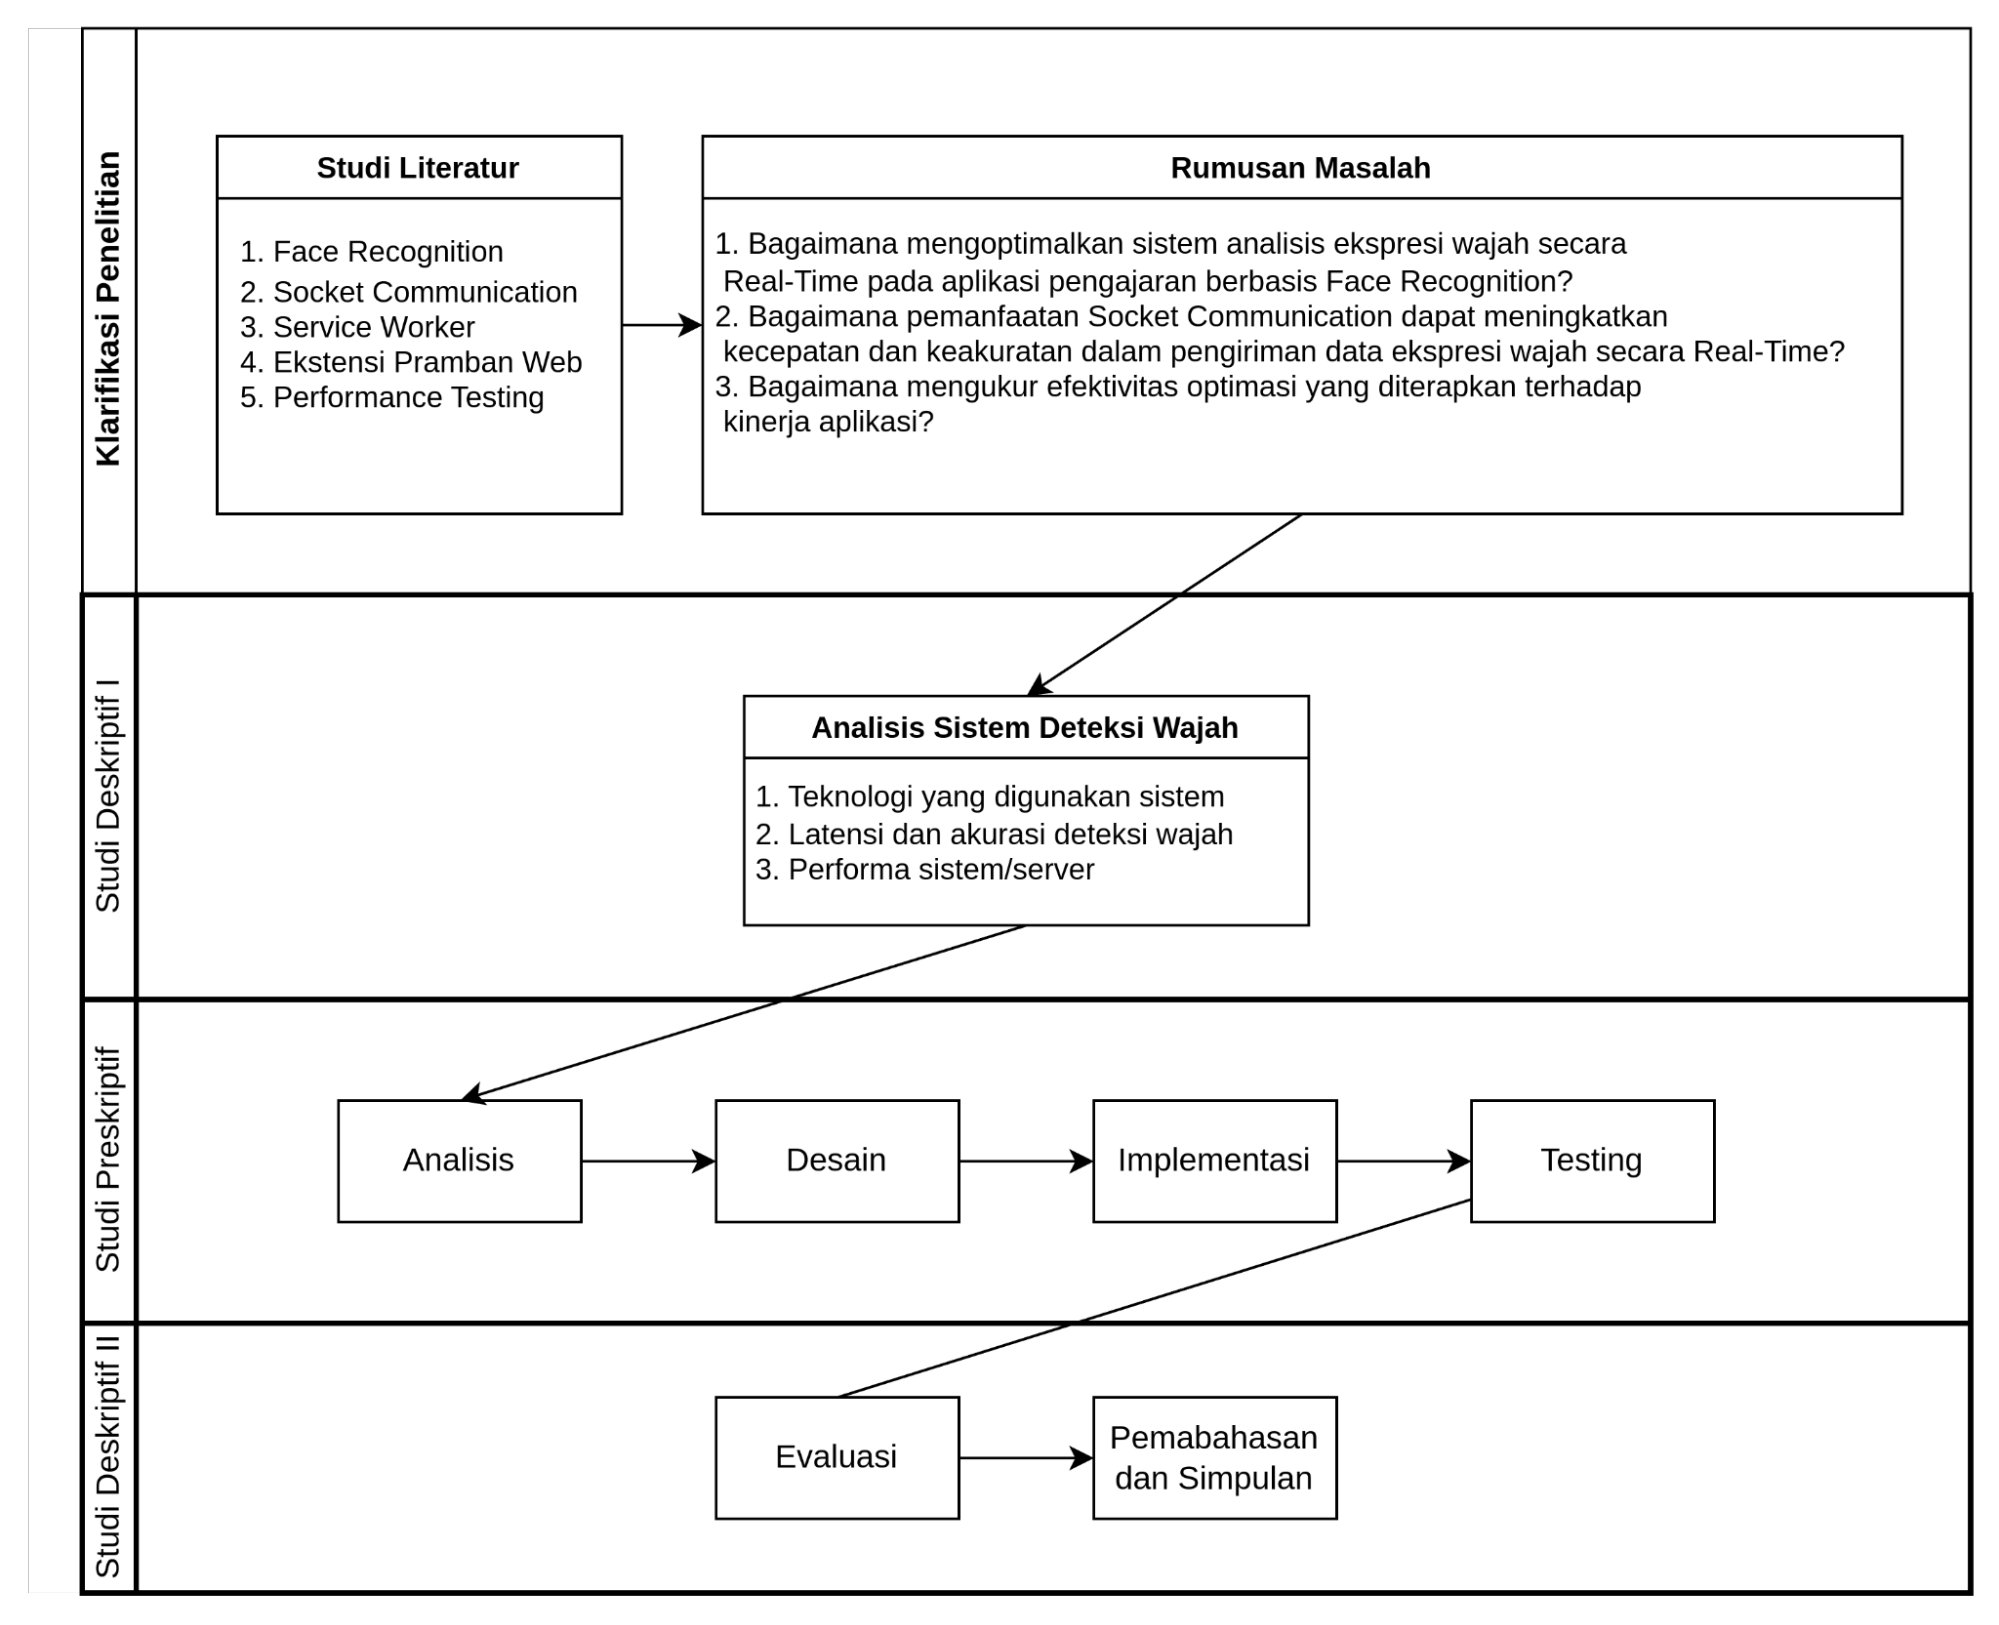
\includegraphics[
    width=14.5cm,
    height=13.5cm,
  ]{images/drm.png}
  \caption{Design Research Methodology (DRM)}
\end{figure}

Penelitian ini menggunakan pendekatan Design Research Methodology (DRM) untuk mengembangkan solusi teknis secara sistematis.
Tujuan utamanya adalah merancang, mengimplementasikan, dan mengevaluasi arsitektur sistem untuk aplikasi EMODU di Google Cloud Platform (GCP).
Melalui DRM, penelitian berfokus pada perancangan arsitektur yang memenuhi tiga pilar utama: ketersediaan tinggi (\textit{high availability}), skalabilitas otomatis (\textit{scalability}), dan penerapan tanpa henti (\textit{zero-downtime deployment}).

\subsection{Klarifikasi Penelitian}
Tahap ini berfokus pada identifikasi masalah dan penentuan ruang lingkup penelitian.
Masalah utama yang diidentifikasi adalah bagaimana membangun infrastruktur yang andal dan efisien untuk aplikasi EMODU, yang berpotensi mengalami pertumbuhan pengguna dan beban kerja yang fluktuatif.
Ruang lingkup penelitian dibatasi pada perancangan dan implementasi arsitektur di Google Cloud Platform (GCP).
Kajian pustaka akan difokuskan pada konsep-konsep kunci seperti arsitektur \textit{high availability}, mekanisme \textit{scalability} pada GCP (misalnya, Managed Instance Groups), strategi \textit{zero-downtime deployment} (seperti Blue-Green atau Rolling Updates), dan praktik terbaik DevOps untuk CI/CD.

\subsection{Studi Deskriptif I}
Pada tahap ini, dilakukan analisis terhadap arsitektur awal atau baseline dari aplikasi EMODU.
Tujuannya adalah untuk memahami komponen-komponen sistem yang ada (backend NestJS, CMS Next.js, komunikasi socket) dan mengidentifikasi potensi kelemahan infrastruktur.
Analisis ini mencakup identifikasi titik tunggal kegagalan (\textit{single points of failure}), potensi masalah skalabilitas, dan proses deployment yang masih manual.
Hasil dari studi ini akan menjadi dasar untuk perancangan arsitektur yang lebih tangguh dan otomatis.

\subsection{Studi Preskriptif}
Pada tahap ini, dirancang sebuah arsitektur infrastruktur solusi di Google Cloud Platform (GCP) untuk mengatasi masalah yang telah diidentifikasi.
Desain arsitektur akan merinci penggunaan layanan-layanan GCP yang spesifik, seperti Google Compute Engine dengan Managed Instance Groups untuk \textit{scaling}, Cloud Load Balancing untuk distribusi lalu lintas dan \textit{high availability}, serta Cloud Build atau GitHub Actions untuk membangun pipeline CI/CD yang mendukung \textit{zero-downtime deployment}.
Arsitektur ini dirancang secara eksplisit untuk memastikan sistem dapat pulih dari kegagalan, beradaptasi dengan beban pengguna, dan dapat diperbarui tanpa mengganggu layanan.

\subsection{Studi Deskriptif II}
Pada tahap ini, arsitektur yang telah dirancang akan diimplementasikan dan dievaluasi kinerjanya.
Aplikasi EMODU akan di-deploy pada infrastruktur GCP yang baru, kemudian serangkaian pengujian akan dilakukan untuk memvalidasi pencapaian tujuan penelitian.
Evaluasi akan mencakup:
\begin{itemize}
    \item \textbf{Pengujian High Availability:} Melakukan simulasi kegagalan (contoh: menghentikan salah satu instance server) dan mengukur waktu pemulihan sistem secara otomatis.
    \item \textbf{Pengujian scalability:} Menggunakan alat \textit{load testing} seperti JMeter untuk memberikan beban lalu lintas yang tinggi dan memverifikasi bahwa sistem secara otomatis menambah atau mengurangi jumlah instance sesuai dengan beban.
    \item \textbf{Pengujian Zero-Downtime Deployment:} Menjalankan pipeline deployment untuk versi baru aplikasi dan memverifikasi bahwa tidak ada gangguan layanan atau kegagalan permintaan selama proses pembaruan.
\end{itemize}
Hasil dari evaluasi ini akan menunjukkan efektivitas dari arsitektur yang diimplementasikan.

\section{Populasi dan Sampel}
Fokus penelitian ini adalah pada sistem teknis, bukan pada pengguna manusia.
Dengan demikian, \textbf{populasi} dalam penelitian ini adalah keseluruhan kemungkinan konfigurasi arsitektur infrastruktur untuk aplikasi berskala seperti EMODU.
\textbf{Sampel} yang diambil adalah arsitektur spesifik yang dirancang dan diimplementasikan pada Google Cloud Platform dalam penelitian ini.
Objek yang diuji bukanlah partisipan manusia, melainkan kinerja dari komponen-komponen infrastruktur itu sendiri ketika diberikan beban kerja yang disimulasikan.

\section{Alat dan Bahan Penelitian}
\subsection{Alat Penelitian}
Spesifikasi komputer yang digunakan untuk pengembangan dan pengelolaan adalah sebagai berikut:
\begin{itemize}
  \item CPU AMD Ryzen 5 PRO 5650U
  \item RAM 14.94 GB
  \item SSD 256 GB
\end{itemize}

\hspace{-32pt} Perangkat lunak yang akan digunakan dalam penelitian ini meliputi:
\begin{itemize}
  \item Fedora Workstation 41
  \item Node.js, NestJS, ReactJS (untuk aplikasi EMODU)
  \item Docker (untuk kontainerisasi aplikasi)
  \item Google Cloud SDK (gcloud CLI)
  \item Postman (untuk pengujian API)
  \item JMeter (untuk \textit{load testing})
  \item Playwright (untuk pengujian \textit{end-to-end})
  \item Grafana \& Google Cloud Monitoring (untuk observabilitas dan visualisasi metrik)
  \item GitHub Actions (untuk pipeline CI/CD)
  \item Zotero, LaTex, Visual Studio Code
\end{itemize}

\hspace{-32pt} Infrastruktur \textit{cloud} yang digunakan dalam penelitian ini adalah \textbf{Google Cloud Platform (GCP)}. Layanan utama yang akan digunakan meliputi:
\begin{itemize}
  \item \textbf{Google Compute Engine (GCE):} Sebagai penyedia mesin virtual untuk menjalankan aplikasi.
  \item \textbf{Managed Instance Groups (MIGs):} Untuk mengelola grup instance dan menerapkan \textit{scaling}.
  \item \textbf{Cloud Load Balancing:} Untuk mendistribusikan lalu lintas dan menyediakan satu titik akses yang \textit{highly available}.
  \item \textbf{Cloud Build:} Sebagai platform CI/CD untuk otomatisasi build, test, dan deploy.
  \item \textbf{Artifact Registry:} Untuk menyimpan dan mengelola artefak build seperti image Docker.
\end{itemize}

\subsection{Bahan Penelitian}
Bahan penelitian yang digunakan meliputi sumber-sumber literatur teknis, yaitu: artikel jurnal ilmiah, dokumentasi resmi dari Google Cloud Platform, buku, dan panduan praktik terbaik (\textit{best practices}) yang berkaitan dengan arsitektur \textit{high availability}, \textit{scalability}, dan \textit{zero-downtime deployment}.
Selain itu, data utama yang menjadi bahan penelitian adalah data kuantitatif berupa metrik kinerja sistem (misalnya, waktu respons, tingkat kesalahan, utilisasi CPU, jumlah instance) yang dikumpulkan dari hasil pengujian beban dan pemantauan sistem.

\section{Instrumen Penelitian}
Instrumen yang digunakan dalam penelitian ini adalah alat untuk membangun, mengukur, dan mengevaluasi arsitektur sistem.
Instrumen utama adalah \textbf{arsitektur infrastruktur itu sendiri} yang diimplementasikan di GCP.
Untuk mengukur kinerja arsitektur tersebut, digunakan instrumen-instrumen berikut:
\begin{itemize}
    \item \textbf{JMeter dan Playwright:} Digunakan sebagai instrumen \textit{load testing} untuk menghasilkan beban pengguna sintetis dan mengukur metrik kinerja seperti \textit{throughput} dan latensi.
    \item \textbf{Google Cloud Monitoring dan Grafana:} Digunakan sebagai instrumen observabilitas untuk mengumpulkan, memantau, dan memvisualisasikan data metrik dari infrastruktur secara \textit{real-time}, seperti utilisasi CPU, jumlah instance, dan status \textit{health check}.
    \item \textbf{Pipeline CI/CD (GitHub Actions/Cloud Build):} Digunakan sebagai instrumen untuk menguji dan memvalidasi proses \textit{zero-downtime deployment}.
    \item \textbf{Skrip Otomatisasi:} Skrip yang dibuat untuk mensimulasikan kegagalan (fault injection), misalnya mematikan instance secara acak, untuk menguji mekanisme \textit{high availability} dan \textit{-failover}.
\end{itemize}
Kombinasi instrumen ini memungkinkan pengumpulan data yang objektif untuk mengevaluasi keberhasilan implementasi arsitektur.

\section{Analisis Data}
Analisis data dalam penelitian ini bersifat kuantitatif dan berfokus pada metrik kinerja infrastruktur yang telah dikumpulkan.
Data akan dianalisis untuk mengevaluasi setiap tujuan utama penelitian:
\begin{itemize}
    \item \textbf{Analisis Scalability:} Menganalisis grafik korelasi antara peningkatan beban (jumlah pengguna virtual) dengan metrik seperti waktu respons dan jumlah instance server yang aktif. Keberhasilan dinilai dari kemampuan sistem menjaga waktu respons tetap stabil dengan menyesuaikan jumlah instance secara otomatis.
    \item \textbf{Analisis High Availability:} Menganalisis log dan data monitoring untuk mengukur waktu yang dibutuhkan sistem untuk pulih setelah simulasi kegagalan. Keberhasilan diukur dari kecepatan pemulihan dan minimnya tingkat kesalahan selama proses \textit{failover}.
    \item \textbf{Analisis Zero-Downtime Deployment:} Menganalisis metrik ketersediaan (availability) dan tingkat kesalahan (error rate) selama proses deployment. Keberhasilan dinilai jika metrik menunjukkan 100\% ketersediaan dan 0\% kesalahan selama pembaruan berlangsung.
\end{itemize}
Hasil analisis ini akan menjadi dasar untuk menarik kesimpulan mengenai efektivitas arsitektur yang diusulkan dalam mencapai \textit{high availability}, \textit{scalability}, dan \textit{zero-downtime deployment}.

\include{contents/chapter4.tex}
\include{contents/chapter5.tex}

% ----------------------------------------
% Daftar pustaka
% ----------------------------------------
\nocite{*}
\printbibliography[heading=bibintoc, title=DAFTAR PUSTAKA]

% ----------------------------------------
% Lampiran
% ----------------------------------------
% https://tex.stackexchange.com/questions/26732/how-to-get-a-list-of-appendices

\end{document}
